%%%%%%%%%%%%%%%%%%%%%%%%%%%%%%%%%%%%%%%%%%%%%%%%%%%%%%%%%%%%%%%%%%%%%%%%%%%%%%%

%%%%%%%%%%%%%%%%%%%%%%%%%%%%%%%%%%%%%%%%%%%%%%%%%%%%%%%%%%%%%%%%%%%%%%%%%%%%%%%

\documentclass[
%   ngerman          % neue deutsche Rechtschreibung
  ,a4paper          % Papiergrösse
% ,twoside          % Zweiseitiger Druck (rechts/links)
% ,10pt             % Schriftgrösse
% ,11pt
  ,12pt
  ,pdftex
%  ,disable         % Todo-Markierungen auschalten
]{report}

% Bitte die Codierung Ihrer Dateien auswählen:
% \usepackage[latin1]{inputenc}    % Für UNIX mit ISO-LATIN-codierten Dateien
% \usepackage[applemac]{inputenc}  % Für Apple Mac
% \usepackage[ansinew]{inputenc}   % Für Microsoft Windows
\usepackage[utf8]{inputenc}        % UTF-8 codierte Dateien
                                   % Dieses Dokument ist unter Unix erstellt, daher
                                   % wird diese Input-Codierung benutzt.


\usepackage{bericht}
\usepackage{acronym}
\usepackage{listings}
\usepackage[sfdefault]{arimo}
\usepackage[ngerman]{babel}
\usepackage[T1]{fontenc}
\usepackage{inconsolata}
\usepackage[onehalfspacing]{setspace}
\usepackage{microtype}				% verbesserter Randausgleich
\usepackage[square, numbers]{natbib}        % natbib als Bibliothek
\bibliographystyle{unsrtnat}                % Nummerische Stil Zitate werden nur mit einer Nummer referenziert
%       unsrtnat, abbrvnat                  % Numerische Stile sortiert und unsortiert
% mehr Infos zu natbib:  https://www.overleaf.com/learn/latex/bibliography_management_with_natbib
\usepackage{nonfloat}               % sollte keine Gleitumgebung geben

\usepackage{fancyhdr}
\pagestyle{fancy}
\fancyhf{} % löscht Kopf- und Fußzeile
\fancyfoot[C]{\thepage} % Seitenzahl unten zentriert
\renewcommand{\headrulewidth}{0pt}

%%%%%%%%%%%%%%%%%%%%%%%%%%%%%%%%%%%%%%%%%%%%%%%%%%%%%%%%%%%%%%%%%%%%%%%%%%%%%%%
%% Angaben zur Arbeit
%%%%%%%%%%%%%%%%%%%%%%%%%%%%%%%%%%%%%%%%%%%%%%%%%%%%%%%%%%%%%%%%%%%%%%%%%%%%%%%

\newcommand{\Autoren}{Kira Isenberg, Fabian Hagenmeier}
\newcommand{\MatrikelNummer}{3427985, 2207087}
\newcommand{\Kursbezeichnung}{TINF22B1}

%%%%%%%%%%%%%%%%%%%%%%%%%%%%%%%%%%%%%%%%%%%%%%%%%%%%%%%%%%%%%%%%%%%%%%%%%%%%%%%%%%%%%

\newcommand{\Was}{Backend für eine Pflanzenpflege-Management-Plattform}
% Wird auf dem Deckblatt in der Erklärung benutzt

%%%%%%%%%%%%%%%%%%%%%%%%%%%%%%%%%%%%%%%%%%%%%%%%%%%%%%%%%%%%%%%%%%%%%%%%%%%%%%%%%%%%%

\newcommand{\Titel}{Programmentwurf - ASWE}
\newcommand{\AbgabeDatum}{31.05.2025}

\newcommand{\Studiengang}{Informatik}

\newcommand{\Studienrichtung}{Medizinische Informatik}
% \newcommand{\Studiengang}{Angewandte Informatik}

%hyperhyper
%howmuchisthefish
\hypersetup{%%
	pdfauthor={\Autoren},
	pdftitle={\Titel},
	pdfsubject={\Was}
}

%%%%%%%%%%%%%%%%%%%%%%%%%%%%%%%%%%%%%%%%%%%%%%%%%%%%%%%%%%%%%%%%%%%%%%%%%%%%%%%
\setlength{\parskip}{0.5em}
\setlength{\parindent}{0pt}
%%%%%%%%%%%%%%%%%%%%%%%%%%%%%%%%%%%%%%%%%%%%%%%%%%%%%%%%%%%%%%%%%%%%%%%%%%%%%%%
\begin{document}
\pagenumbering{roman}
%%%%%%%%%%%%%%%%%%%%%%%%%%%%%%%%%%%%%%%%%%%%%%%%%%%%%%%%%%%%%%%%%%%%%%%%%%%%%%%
% Titelseite, Hier muss man nichts ändern

\begin{titlepage}
\begin{center}
	\vspace*{-2cm}
	\hfill
\includegraphics[width=4cm]{img/dhbw-logo}\\[2cm]
	{\Huge \Titel}\\[1.5cm]
	{\Huge\scshape \Was}\\[1.5cm]
	{\large Studienrichtung \Studienrichtung}\\[0.5cm]
	{\large an der}\\[0.5cm]
	{\large Dualen Hochschule Baden-Württemberg Karlsruhe}\\[0.5cm]

	\vfill
\end{center}
\begin{tabular}{l@{\hspace{2cm}}l}
Studenten	                    & \Autoren		\\
Matrikelnummern	                & \MatrikelNummer		\\
Kurs			         		& \Kursbezeichnung		\\
Abgabedatum               		& \AbgabeDatum		    \\
Dozent			         		& Daniel Lindner		\\

\end{tabular}
\end{titlepage}
\onehalfspacing



\newpage
\tableofcontents           % Inhaltsverzeichnis hier ausgeben
\listoffigures             % Liste der Abbildungen
%\listoftables              % Liste der Tabellen
%\lstlistoflistings         % Liste der Listings
%\listofequations           % Liste der Formeln

% Jetzt kommt der "eigentliche" Text

%%%%%%%%%%%%%%%%%%%%%%%%%%%%%%%%%%%%%%%%%%%%%%%%%%%%%%%%%%%%%%%%%%%%%%%%%%%%%%%
%       Vorlage Abkürzungsverzeichnis
%%%%%%%%%%%%%%%%%%%%%%%%%%%%%%%%%%%%%%%%%%%%%%%%%%%%%%%%%%%%%%%%%%%%%%%%%%%%%%%

\chapter*{Abkürzungsverzeichnis}        
% chapter*{..} -->   keine Nummer, kein "Kapitel"
% Wird dadurch nicht ins Inhaltsverzeichnis eingetragen

% Damit das doch ins Inhaltsverzeichnis kommt
% \addcontentsline{toc}{chapter}{Akürzungsverzeichnis}   

%%%%%%%%%%%%%%%%%%%%%%%%%%%%%%%%%%%%%%%%%%%%%%%%%%%%%%%%%%%%%%%%%%%%%%%%%%%%%%%%
% Hier werden die Abkürzungen definiert
% \acro{Name}{Darstellung der Abkürzung}{Langform der Abkürzung}
 % Folgendes benutzen, wenn der Plural einer Abk. benöigt wird
 % \newacroplural{Name}{Darstellung der Abkürzung}{Langform der Abkürzung}
 % Wenn nicht benutzt, erscheint diese Abk. nicht in der Liste
%%%%%%%%%%%%%%%%%%%%%%%%%%%%%%%%%%%%%%%%%%%%%%%%%%%%%%%%%%%%%%%%%%%%%%%%%%%%%%%% 
\begin{acronym}[OPC-UA]

%.	
\acro{.NET}[.NET]{.NET von Mircorsoft}
%A
\acro{Add-On}[Add-On]{Plug-in, Software-Erweiterungen}
\acro{Agilent}[Agilent]{Agilent Technologies}
\acro{ARM}[ARM]{Advanced RISC Machine}
\acro{API}[API]{Application-Programming-Interfaces}
%B
\acro{bzw.}[bzw.]{beziehungsweise}
%C
\acro{CDS}[CDS]{Chromatograpy Data System}
\acro{CE}[CE]{Kapillarelektrophorese}
\acro{COM}[COM]{Component Object Model}
\acro{CRM}[CRM]{Customer Relationship Management}

\acro{CPU}[CPU]{Central Processing Unit}
%D
\acro{DSL}[DSL]{Domain Specific Language}
%E
\acro{ELK}[ELK]{Elasticsearch, Logstash und Kibana}
\acro{ETL}[ETL]{Extract, Transform and Load}
%F

%G

%H
\acro{HP}[HP]{Hewlett-Peckard}
\acro{HPLC}[HPLC]{Hochleistungsflüssigkeitschromatographen}
\acro{http}[http]{Hypertext Transfer Protocol}
%I
\acro{IoT}[IoT]{Internet of Things}
\acro{IP}[IP]{Internet Protocol}
%J
\acro{JSON}[JSON]{JavaScript Object Notation}
%K
%L
\acro{LC}[LC]{Flüssigkeitschromatographen}
\acro{LINQ}[LINQ]{Language Integrated Query}
%M
\acro{MIT}[MIT]{Massachusetts Institute of Technology}
%N
\acro{NoSQL}[NoSQL]{non-relational oder Not only SQL}
%O
%P
\acro{PHP}[PHP]{Hypertext Preprocessor}
\acro{Plug-in}[Plug-in]{Software-Erweiterungen}
\acro{PL29}[PL29]{Product Line 29}
%Q
%R
\acro{RESTful}[RESTful]{Representational State Transfer}
%S
\acro{SDK}[SDK]{Software Development Kit}
\acro{SID}[SID]{Software Informatik Division}
\acro{SQL}[SQL]{Structured Query Language/Strukturierte Abfrage Sprache}
%T
%U
\acro{UTF}[UTF]{Unicode Transformation Format}
%V
%W
%X
\acro{XML}[XML]{Extensible Markup Language}
%Y
\acro{YAML}[YAML]{YAML Ain't Markup Language}
%Z
\acro{z.B.}[z.B.]{zum Beispiel}
%123

%%%%%%%%%%%%%%%%%%%%%%%%%%%%%%%%%%%%%%%%%%%%%%%%%%%%%%%%%%%%%%%%%%%%%%%%%%%%%%
%       Wie im Text zitieren??
%%%%%%%%%%%%%%%%%%%%%%%%%%%%%%%%%%%%%%%%%%%%%%%%%%%%%%%%%%%%%%%%%%%%%%%%%%%%%%
% \ac{name}         Nur die Abkürzung wird referenziert
% \acs{name}        Langform mit Abkürzung in Klammer


\end{acronym}
              % Abkürzungsverzeichnis
\pagenumbering{arabic}

%%%%%%%%%%%%%%%%%%%%%%%%%%%%%%%%%%%%%%%%%%%%%%%%%%%
\chapter{Einleitung}
%%%%%%%%%%%%%%%%%%%%%%%%%%%%%%%%%%%%%%%%%%%%%%%%%%%
Die Idee zu diesem Projekt entstand aus einem ganz persönlichen Bedürfnis: Kira möchte langfristig ein System entwickeln, mit dem sie die
Pflanzen in ihrem hydroponischen Garten verwalten kann. Statt sich alleine durch ein großes Softwareprojekt zu kämpfen, haben wir die
Gelegenheit genutzt, diese Idee mit dem Programmentwurf zu verbinden – und damit die Grundlage für eine spätere, vollständige Anwendung
geschaffen.

Unser Ziel war es nicht, eine fertige App abzuliefern, sondern ein robustes, erweiterbares Backend zu entwickeln, das zentrale Funktionen wie
die Verwaltung von Pflanzen, Pflegeplänen und Pflegeaufgaben unterstützt. Dabei haben wir besonderen Wert auf eine saubere Strukturierung nach
den Prinzipien der Clean Architecture, testbare Komponenten und sinnvolle Domain-Modelle gelegt – alles mit dem Ziel, das System später
problemlos erweitern zu können.

Der Abschnitt zu Unit Tests soll doppelt gewertet werden.

Unsere Codebasis ist unter https://github.com/kira-isi/plant-care-backend öffentlich zugänglich.
%%%%%%%%%%%%%%%%%%%%%%%%%%%%%%%%%%%%%%%%%%%%%%%%%%%%%%%%%%%%%%%%%%%%%%%%%%%%%%%%%%%
\chapter{Grundlagen}
%%%%%%%%%%%%%%%%%%%%%%%%%%%%%%%%%%%%%%%%%%%%%%%%%%%%%%%%%%%%%%%%%%%%%%%%%%%%%%%%%%%
\section{Grundlegende Bausteine}
% [h]       sollte die Tabelle genau hier anzeigen
% {clrp}    sind verschieden parameter zum eanzeigen der Tabelle
%           Anzahl der Buchstaben gleich Anzahl der Spalten
%           c           zentrierter Text
%           r           rechtsbündiger Text
%           l           linksbündiger Text
%           p{"x"cm}    Spalte soll "x" cm breit sein
%           |           fügt einen senkrechten Strich zwischen den Spalten ein
%           \hline      Horizontale Linie ober/unter und zwischen den Zeilen einfügen für Umrandung der Zellen 
%           \\          Trennung der Zeilen
%           &           Trennung der Spalten 

\subsection{Wie baut man Tabellen?}

Hier ganz viel Text und eine Referenz auf die Tabelle \ref{tab:heisetabelle}. 
\begin{table}[h]
	\begin{tabular}[h]{|l|p{7cm}|}
	%\caption{Beschreibung der Tabelle}
	    \hline
		erste Spalte und Zeile & zweite Spalte und erste Zeile \\
		\hline
		erste Spalte und zweite Zeile & zweite Spalte und zweite Zeile \\
		erste Spalte und dritte Zeile & zweite Spalte und dritte Zeile \\
		\label{tab:heisetabelle}
	\end{tabular}
\end{table}

\subsection{Wie erstellt man eine Aufzählung?}

Beispiele für Klassifizierungsprobleme:
\begin{itemize}
    \item Handschrifterkennung
    \item Krankheitsanalyse
    \item E-Mail Spamfilter
\end{itemize}

\subsection{Bissl Mathe Nötig?}

\begin{displaymath}
    logit(p) = log \frac{p}{(1-p)}
    logit(p(y=1|x)) = \sum_{i=0}^{m} w_{i}x_{i} = w^T x 
\end{displaymath}

\begin{displaymath}
    \hat{y} =\left\{%
    \begin{array}{lll}
        1, & wenn & sig(z) \ge 0.5\\
        0, & andernfalls & \\
    \end{array}%
    \right.
\end{displaymath}

\section*{Hier eine Section ohne Nummerierung}

\subsection*{Geht auch bei Subsections}
Das funktioniert einfach in dem man ein Stern zwischen sub/section und den {} setzt.
\subsection{Und wieder mit Nummern}
Aber wie ihr seht werden die Nummern nicht einfach ausgeblendet sondern gar nicht erst erstellt, somit geht es hier weiter mit 2.1.4 was theoretisch 2.2.2 sein müsste.

Nummern wegzulassen ist meiner Meinung nur Sinnvoll wenn Ihr zum Beispiel alle Subsections nicht auflisten wollt, da wenn die Nummerierung wegelassen wird, diese sectionen auch nicht im Inhaltsverzeichnis auftauchen. Bei subsections macht es daher Sinn, wenn das Inhaltsverzeichnis zu groß wird oder die subsections für das Inhaltsverzeichnis uninteressant sind. Hier noch ein kleines Beispiel wie am Absätze macht. Entweder einfach eine Zeile freilassen 

oder zwei \\  Backslashs schreiben 
%%%%%%%%%%%%%%%%%%%%%%%%%%%%%%%%%%%%%%%%%%%%%%%%%%%%%%%%%%%%%%%%%%%%%%%%%%%%%%%%%%%
\chapter{Unit-Tests}
\section{Ziel und Aufbau der Tests}
Ziel unserer Tests war nicht die vollständige Abdeckung aller Programmteile, sondern das exemplarische Aufzeigen, wie Unit-Tests im Rahmen einer
sauberen Architektur sinnvoll eingesetzt werden können. Im Mittelpunkt standen daher ausgewählte, fachlich relevante Methoden und Use Cases.

Wir haben uns darauf konzentriert, die Logik in der Domain- und Application-Schicht zu testen. Die Tests wurden mit xUnit geschrieben und folgen
durchgehend dem Arrange-Act-Assert-Muster.

Insgesamt wurden 11 Unit-Tests erstellt. Diese decken zentrale Bereiche der Domain- und Application-Schicht ab:

\begin{itemize}
    \item CareTaskTests: Fälligkeitsprüfung bei wiederkehrenden Aufgaben
    \item LocationTests: Validierung und Anlage von Standorten
    \item PlantTests: Erstellung und Aktualisierung von Pflanzen
\end{itemize}

Von 11 Tests waren 8 auf anhieb erfolgreich. Debei viel auf das besonders fehlerhafte Eingaben wie leere Strings in usecases und Konstrucktoren nicht
beachtet wurden.

\begin{figure}[H]
\centering
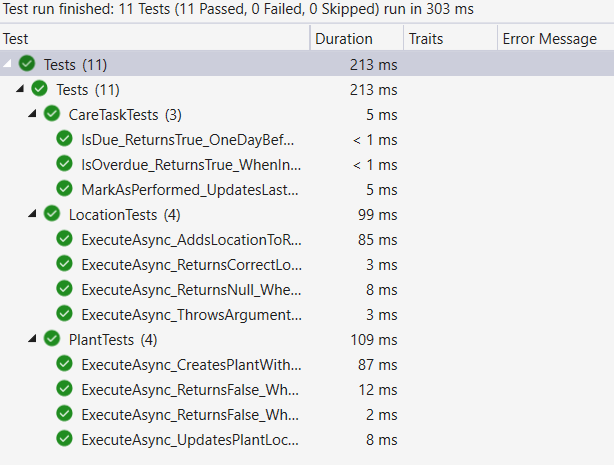
\includegraphics[width=0.50\textwidth]{img/tests.png}
\caption{Erfolgreicher Test-Durchlauf}
\end{figure}

\section{Einsatz von Mocks}
Um Use Cases isoliert zu testen, kamen Mocks zum Einsatz – erstellt mit dem Framework Moq. So konnten Repository-Interfaces ersetzt und typische
Szenarien simuliert werden wie etwa eine Abfrage, die ein bestimmtes Domain-Objekt zurückliefert oder die Prüfung, ob ein AddAsync-Aufruf mit
den erwarteten Daten erfolgt. Die Mocks ermöglichen saubere Unit-Tests ohne externe Infrastruktur.

Die Implementierungen der Repositories selbst wurden nicht getestet, da diese als Integrationstests zu werten wären und nicht zum Fokus eines Programmentwurfs im Sinne der Clean Architecture gehören.

\section{Teststrategie und Abdeckung}
Die Testabdeckung wurde mit Coverlet gemessen. Der Gesamtwert beträgt 15,3 \%, was angesichts der gezielten Auswahl und des prototypischen Charakters des Projekts erwartbar war.
Es wurden nur sehr wenige kleine Aspekte der Anwendung getestet. Komplexe Controller sind nicht implementiert und konnten daher auch nicht getestet werden.

Viele Zeilen entfallen zudem auf DTOs, Konfigurationen oder technische Infrastruktur (z. B. Datenbankadapter).

\begin{figure}[H]
\centering
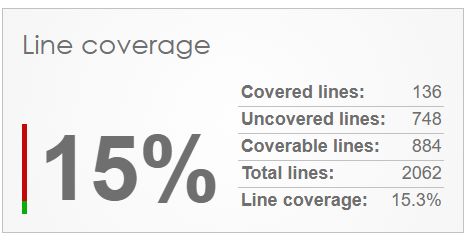
\includegraphics[width=0.50\textwidth]{img/coverage.png}
\caption{Coverrage durch Unit-Tests}
\end{figure}

Die Tests dienten dabei auch zur Reflektion der Architektur: Wiederverwendbarkeit, Testbarkeit und Trennung von Zuständigkeiten. Sie helfen den Entwicklungsprozess aktiv zu hinterfragten und zu verbessern.

\section{ATRIP-Analyse}
Unsere Tests erfüllen die ATRIP-Kriterien im Rahmen des Programmentwurfs in sinnvoller Weise.

\begin{itemize}
    \item Automatic: Alle Tests sind vollständig automatisiert mit xUnit eingebunden. Sie lassen sich ohne manuelle Schritte per dotnet test ausführen.
Auch die Code Coverage wurde über Coverlet integriert, was den automatisierten Testprozess sinnvoll ergänzt.
    \item Thorough: Wir haben nicht alle relevanten Funktionen getestet – insbesondere Randfälle, Validierungslogik und Fehlerbehandlung wurden
größtenteils ausgespart. Das war allerdings eine bewusste Entscheidung. Stattdessen haben wir exemplarisch zentrale fachliche Methoden getestet,
z. B. die Fälligkeitsprüfung bei Pflegeaufgaben oder das Erstellen und Aktualisieren von Pflanzen. Die Tests zeigen, dass unser Code testbar
aufgebaut ist, auch wenn nicht alle Fälle abgedeckt sind.
    \item Repeatable: Alle Tests laufen stabil und liefern reproduzierbare Ergebnisse. Es gibt keine externe Abhängigkeit (z. B. Datenbank), weil alle
Infrastrukturkomponenten gemockt wurden. Ein Beispiel ist CreatePlant, bei dem das Repository vollständig isoliert und das Verhalten überprüfbar
ist.
    \item Independent: Unsere Tests sind voneinander unabhängig. Jeder Test initialisiert seine eigene Datenbasis, es gibt keine gemeinsame Setup-Logik
oder globale Zustände. Das gilt sowohl für einfache Domain-Methoden als auch für die Use Cases.
    \item Professional: Die Tests sind klar benannt und strukturiert. Wir folgen durchgängig dem AAA-Muster.
\end{itemize}

\begin{figure}[H]
\centering
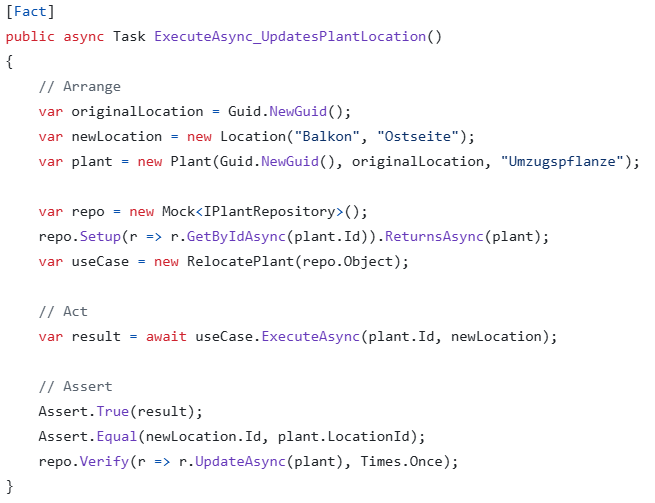
\includegraphics[width=1.00\textwidth]{img/test.png}
\caption{Beispiel für einen Test}
\end{figure}
% !TeX spellcheck = de_DE
\chapter{Domain Driven Design}
Unsere Domäne ist die Pflanzenpflege, ein Bereich, der nicht unbedingt gut professionell durchorganisiert ist. Und trotzdem enthält diese Domäne Begriffe und Aktionen, die sich durch die Gesamtheit der Tätigkeit ziehen. Für dieses Projekt wurde es vorgezogen, die Domänensprache im Code auf Englisch anzuwenden, deshalb würd für jeden deutschen Domänenbegriff die im code verwendete englische Übersetzung in Klammern zugefügt.

\subsection*{Entitäten}
Ganz im Vordergrund stehen hier 3 Dinge, die Pflanze selbst, die Pflegeaktionen und die Organisation dieser in einem Plan.
\par
Pflanzen sind das Hauptobjekt der Domäne. Pflanzen sind meist durch Ihren Artennamen spezifiziert. Arten teilen bestimmte Merkmale miteinander, wie zum Beispiel wann und wie viel Wasser oder Sonne sie benötigen. Bewässerung kann manuell als Aktion durchgeführt werden.  Das nötige Sonnenlicht erhalten die Pflanzen meist durch ihre Platzierung an sonnigeren oder schattigeren Bereichen. 
\par
Es gibt verschiedene Typen von Aktionen. Einmalige Tasks werden einmalig geplant und durchgeführt, wiederkehrende Aufgaben werden in einem gegebenen Zeitintervall wiederholt. Daraus ergeben sich zwei weitere Entitäten für die Domäne, die die Pflegeaktion spezifizieren.
\par
Daraus Ergeben sich die Hauptsächlichen Entitäten, die in der Domäne abgebildet werden sollen:

\begin{itemize}
	\item Pflanze und Pflanzentyp (Plant und PlantType)
	\item Platzierung (Location)
	\item Pflegeaktion (CareTask)
	\item Einmalige, geplante Aktion (ScheduledTask)
	\item Wiederkehrende Aufgabe (RecurringTask)
\end{itemize}

\subsection*{Value Objects}
Pflegeaktionen kommen in unterschiedlichen Typen, die sich allerdings in ihrer Art auch bei Anwendung auf verschiedene Pflanzentypen eigentlich nicht ändern. Deshalb werden die einzelnen Pflegeaktionen als ValueObjects in der Domäne angesehen. Sie besitzen durch ihren Typen eine inhärente Wertigkeit für den Anwender, sind allerdings im Code alle gleich zu behandeln.  Sie benötigen keine besonderen Methoden oder Attribute, ihr größtes Unterscheidungsmerkmal ist der Typ selbst. Pflegeaktionen, die als Value Objects angelegt wurden, beinhalten:

\begin{itemize}
	\item Bewässerung (Watering)
	\item Düngen (Fertilizing)
	\item Umtopfen (Repotting)
	\item Zurückschneiden oder Stutzen (Pruning)
\end{itemize}

Des weiteren existieren in der Domäne noch die Möglichkeit bestimmten Value Objects noch Details anzuhaften. So muss zum Beispiel beim Bewässern klar sein, wie viel Wasser gegeben werden soll, oder welcher Dünger in welcher Menge angewandt werden soll. Dafür wurden die careTaskDetails eingeführt.

\subsection*{Aggregate}
Ein klassisches Beispiel für Aggregate in dieser Domain Bildes der Pflegeplan. Nach der Initialisierung ist es im Pflegeplan möglich, sowohl Pflanzen als auch Aktionen hinzuzufügen und zu entfernen, alle zugewiesenen Aktionen oder Pflanzen zurückzusetzen, sowie alle auszuführenden Aktionen auf einen Blick erkennen zu können. Damit erfüllt der Pflegeplan auch die Anforderungen von CRUD.

\subsection*{Repositories}
In dieser Domäne stellen Repositories eine Sammlung aus entweder Aggregaten oder deren Komponenten da, aus denen über IDs Zugriff gewährt wird. Auch für Locations, die nicht direkt Teil eines Aggregates sind, gibt es ein Interface. Daher gibt es im Code vorbereitete Repositories für Pflanzen, Aktionen und Pflegepläne. Sie werden hauptsächlich verwendet, um Domain Services eine Sammlung an Objekten zu geben, mit denen diese Weiterarbeiten können. Dabei wurden sie nur als Interfaces definiert, um nicht die Generierung und Speicherung nach Außen geben zu können (Stichwort Dependency Injection). 
\par
Die Repositories erben alle von der Parent Interface IGenericRepository, die die Methoden zum Besorgen von Objekten per ID, das Hinzufügen, Updaten und Löschen vorschreiben. 
\par
Für den CarePlan werden zursätzlich noch Methoden vorgeschrieben, die es ermöglichen alle Plane mit Aktionen zu erhalten, die entweder anstehen oder bereits überfällig sind. Für Pflanzen wird vorgeschrieben eine Methode zu implementieren, die es ermöglicht Pflanzen auch per Typ zu finden. Da es sich dabei um keine eindeutige Zuweisung handelt, wird der Return Type der Methode als IEnumerable vorgeschrieben.

\subsection*{Domain Services}
Domain Services bilden Aktionen ab, die im ausführenden Code später die Lesbarkeit erhöhen und diese Aktionen standardisieren.  In der Domäne der Pflanzenpflege gibt es einige Domain Services, die abgebildet werden müssen. Diese lassen sich dabei in 3 Grundarten unterteilen: Pflegeplan-Management (carePlanManagement), Platzierungs-Management (locationManagement) und Pflanzen-Management (plantManagement).
\par
In den Grundarten bilden sich verschiedene Aktionen ab, die alle später durch Verwendung der Domain Services automatisiert durchgeführt werden können, wie zum Beispiel die Domain Services AddTaskToCarePlan oder GetDueTasksForCarePlan. Die lassen den späteren Ausführungscode verboser, im Sinne des Domain Driven Designs, erscheinen.
\par
Innerhalb des Codes überscheiden sich die Domain Services mit dem Prinzip der Use Cases der Clean Architecture und werden deshalb auch als solche betitelt.

% !TeX spellcheck = de_DE
\chapter{Refactoring}

Im Zuge des Refactoring wurde zuerst einmal ein code review durchgeführt. Dabei wurde der gesamte erstellte Code im Repository einmal „mit dem Auge“ auf Auffälligkeiten geprüft, danach ein zweites Mal mit einer Checklist, die Anhand der Vorlesung erstellt wurde. Diese Checkliste beinhaltete die besprochenen Code Smell Beispiele, konkret Duplicated Code, Long Method, large Class, Shotgun Surgery, Switch Statements, Code Comments, geprüft.
Hierbei wurden mehrere, zumeist kleinere Stellen identifiziert, bei denen Ausbesserungsbedarf bestand. Bei diesen Findings handelte es sich um Code Smell Fälle, die wir bereits konkret in der Vorlesung behandelt hatten:
\subsection*{}
\begin{enumerate}
\item Es wurde ein Switch-Statement für die Identifizierung eines Enums verwendet
\item In einem Konkreten Fall eine Methode mit auslagerbarem Code identifiziert („Long Method“)
\item Execute Methoden der Use Cases beinhalteten Error Return Werte
\item Viel ähnlicher Code in Use Case Definitionen
\end{enumerate}
\subsection*{}
Bei weiteren waren minimale Optimierungen anderer Aspekte gefragt, um den Code etwas ausbessern und lesbarer zu machen:
\subsection*{}
\begin{enumerate}
\item[a.] Manche Methodennamen hielten sich nicht an die gängigen C\# Benennungskonventionen (hauptsächlich Großschreibung) oder waren im Sinne des Domain Driven Designs nicht optimal benannt
\item[b.] Manche Variablen konnten den Wert NULL annehmen, waren aber nicht entsprechend konfiguriert
\item[c.] Inkonsistente Variableninitialisierung in Use Cases
\end{enumerate}
\subsection*{}
Diese Findings nach der Identifizierung in einem neuen Zweig des Repositories jeweils einzeln bearbeitet.
\par
Im ersten Finding wurde im Konstruktor der Klasse CareTask eine statische Methode MatchesDetailsType zum identifizieren des Task Typen eines Objektes einer Klasse, die aus dem Interface ICareTaskDetails, also eine detaillierte Pflegeaufgabe. Die Statische Methode verwendete dabei einen Switch Case und iterierte über den Enum-Typen CareType und den passenden Typen der Variable type zu finden. Dabei handelt es sich um ein gutes Besipiel des Code Smells Switch Statements, und damit im einen Shotgun Surgery Smell im erweiterten Sinne. Wird das Enum erweitert, so muss der Entwickler auch wissen, dass dieses Switch Statement exisitert und das er erweitert werden muss, sonst baut ein unwissender Entwickler eine Fehlerquelle in den Code. Um eben nicht bei jeder Erweiterung des Enums CareType auch das Switch Statement der MatchesDetailsType erweitern zu müssen, muss hier deshalb eine Änderung vorgenommen werden.  Der Klassische Lösungsansatz solcher Problematiken ist dabei das Nutzen von Polymorphie um das Switch Statement als Conditional zu ersetzen. Dies wurde auch hier angewandt. 
\par
Dafür wurde das Enum aufgelöst, und jedes Element des Enum zu einer eigenen Klasse umgeschrieben, die alle von einer abstakten ParentKlasse CareType erben. Diese bekommt eine abstrakte Methode Matches zugeordnet, die alle Children implementieren. Dabei wird der CareType des übergebenen Arguments von Typ ICareTaskDetails auf Gleichheit mit dem jeweils eigenen Typen geprüft. So muss in der Kontruktor von CareTask nurnoch vom übergebenen Argument type des Typen CareType die matches methode auf das andere Argument details aufrufen und erhält dasselbe Ergebnis wie zuvor. Wird ein neuer CareType hinzugefügt, muss dies aber nur noch an einer Stelle gemacht werden und der Entwickler braucht keine Kenntnis mehr über die Existens des Switch Cases in der Klasse CareTask.
\subsection*{}
Im zweiten Finding wurde im Use Case CreateCarePlan, in der Execute Methode über eine übergebene Liste von PflanzenIDs iteriert, die korrespondierenden Objekte aus einem Repository-Objekt entnommen und dem CarePlan hinzugefügt. Hierbei handelt es sich um einen Long Method Smell (im engeren Sinne auch um ein Code Comments Smell, da der Block logisch getrennt vom Rest des Methodencodes ist; allerdings gab es hier keine Abtrennung per Kommentar, also trifft der Smell eventuell nicht 100\% zu). Zur Lösung dieses Smells wurde die sogenannte „Extract Method“-Lösung angewandt. 
\par
Dazu wurde der Code aus der Methode heraus separiert und in eine eigene Methode ausgelagert, die mit dem Keyword protected versehen wird, um nur klasseninterne Zugriffe zuzulassen. Der Name der neuen Methode wurde so gewählt, dass das Lesen der Methode Execute im Sinne des Domain Driven Designs möglichst umkompliziert und in der ubiquitous language bleibt. So entstand die Methode FillCarePlanWithPlants, die als Argumente einen CarePlan und eine Liste von PlantIDs erwartet, das Heraussuchen der Pflanzen aus dem Repository übernimmt und den CarePlan damit auffüllt. Anschließend wird der aufgefüllte CarePlan zurückgegeben. 
\subsection*{}
Beim dritten Finding wurde identifiziert, dass viele UseCases, die entweder etwas Löschen oder Ändern sollen, bei einer fehlgeschlagenden Suche des jeweiligen Objektes aus einem Repository als Return-Wert false übergeben, was äquivalent zu einem Fehler angesehen werden kann.  Diese können allerdings auch direkt als Fehler identifiziert und über eine Exception handgehabt werden. Dafür wurde beispielsweise in der ExecuteAsync Methode der use case Klasse AssignPlantToCarePlan eine solche sogenannte „Replace Error Code with Exception“ Lösung umgesetzt. Hierfür wurden neue Exceptions im Domain Code erstellt. Dafür wurde zuerst die Parent Exception NotFoundException kreeirt, und dann die beien Children Exceptions CarePlanNotFoundException und PlantNotFoundException. Diese können dann anstelle einer Wiedergabe von false implmenetiert werden und können durch Ausgabe einer Fehlermeldung über das Argument message verboser das eigentliche Problem beim Ausführen der Methode ansprechen. Diese Implementation könnte auch in Use Case Klassen wie DeleteCarePlan und DeleteTaskFromCarePlan implementiert werden, da auch dort der Fall auftritt, bei nicht-Finden des zu Entfernenden Objektes der Wert false zurückgegeben wird.
\subsection*{}
Im vierten Finding wurde Identifiziert, dass sich der Code, gerade in den Execute bzw ExecuteAsync Methoden vieler Use Cases ähneln. Bei näherer Betrachtung sind diese Methoden allerdings immer leicht unterschiedlich, und sich überschneidende Teile sind minimal. Deshalb wurde von einer Optimierung beispielsweise im Sinne einer Extraktion von Code abgesehen. Da diese wahrscheinlich nur wenige Zeilen code beinhalten und auch beim Leseverständnis nicht unbedingt weiterhelfen würden. Ein weiterer Gedanke zur Optimierung wäre eventuell eine Vererbung, die die Überlappenden Teile in einer Parent Klasse übernimmt. Aber auch hier konnte im Zuge des Refactorings keine zufriedenstellende Umsetzung gefunden werden, die den Code optimiert und das Leseverständnis nicht beeinträchtigt.
\subsection*{}
Bezüglich der kleineren Findings wurde in Finding a bemerkt, dass manche Methoden der CarePlan Klasse mit Kleinbuchstaben beginnen. Konvention bei C\# ist allerdings, Methoden mit Großbuchstaben beginnen zu lassen, was ein kleines Renaming Refactoring zur Folge hatte. Dies gilt dabei auch für Attribute von Klassen, die Getter und Setter definieren.
\par
Zu Finding b lässt sich sagen, dass es in C\# best practice ist, eine Variable, die auch den Wert NULL annehmen können soll, entsprechend zu konfigurieren. Entweder, wenn die Variable gleich mit Inhalt befüllt wird, kann das Keyword var anstatt eines Variablentypen eingesetzt werden. Der Compiler prüft dann auf den Typen der befüllt werden soll, und konfiguriert automatisch die Nullbarkeit der Variable. Dies kann aber auch manuell umgesetzt werden, indem hinter das Keyword des Variablentypen ein Fragezeichen gesetzt wird. So weiß der Compiler, dass für diese Variable auch NULL ein gültiger Wert sein kann.
An vereinzelten Stellen wurde diese Konfiguration vergessen, und im Zuge des Refactorings entsprechend angepasst.
\par
Finding c bezieht sich inhaltlich auf Finding b. So wurden in Use Cases fast durchgängig var Keywords in den Execute Methoden verwendet, vereinzelt aber auch die Typen. Um hier konsistent zu bleiben, und auch um die Nullbarkeit von Finding b zu erhalten, wurde hier auf konstanten Nutzen von var umgestellt.
Nachdem alle Findings bearbeitet, und kleiner Fehler bei der Bearbeitung, wie zum Beispiel eine vergessene Negierung bei der Gleichheitsprüfung von Finding 2, behoben wurden, wurde ein Merge Request vom Nebenzweig auf den Hauptzweig erstellt, nochmals reviewed und gemergt.

 

% !TeX spellcheck = de_DE
\chapter{Fazit}



%%%%%%%%%%%%%%%%%%%%%%%%%%%%%%%%%%%%%%%%%%%%%%%%%%%%%%%%%%%%%%%%%%%%%%%%%%%%%%%%
% Ab hier beginnt der Anhang
%%%%%%%%%%%%%%%%%%%%%%%%%%%%%%%%%%%%%%%%%%%%%%%%%%%%%%%%%%%%%%%%%%%%%%%%%%%%%%%%
%\appendix
%\addcontentsline{toc}{chapter}{Anhang}
%
\chapter*{Anhang}

%\addcontentsline{toc}{chapter}{Index}
%\printindex


%%%%%%%%%%%%%%%%%%%%%%%%%%%%%%%%%%%%%%%%%%%%%%%%%%%%%%%%%%%%%%%%%%%%%%%%%%%%%%%%
% Bibliothek wird hier eingebunden. 

%%%%%%%%%%%%%%%%%%%%%%%%%%%%%%%%%%%%%%%%%%%%%%%%%%%%%%%%%%%%%%%%%%%%%%%%%%%%%%%%

\end{document}

%%%%%%%%%%%%%%%%%%%%%%%%%%%%%%%%%%%%%%%%%%%%%%%%%%%%%%%%%%%%%%%%%%%%%%%%%%%%%%%%
%%%%%%%%%%%%%%%%%%%%%%%%%%%%%%%%%%%%%%%%%%%%%%%%%%%%%%%%%%%%%%%%%%%%%%%%%%%%%%%%
% Nützliche Codes für den Content/Kapitel
%
%   wenn Text über den Rand geht kann man das mit sloppypar
%   \begin{sloppypar}
%       bla bla text...
%   \end{sloppypar}
%   
%   Kursiver Text:
%   \textit{...}
%
%
%
%
%